% Put between [ ] in document class report type following these macros:
%
% + daily
% + weekly
% + monthly

\documentclass[daily]{engenius}

\usepackage{float} % For the 'H' option

\usepackage{xcolor}
\definecolor{myGreen}{RGB}{12,130,21}
\definecolor{myRed}{RGB}{80,15,6}

\titlespacing*{\section}{0pt}{0ex plus 1ex minus 0.2ex}{0ex plus 0.2ex}

% Fill the document parameters
% Remove \titletwo if you want one title
% You can remove authors by deleting then
% You have 3 option for the department identification as showed bellow

\title{Pharma Comp.}
\titletwo

% Use the author section to show some basic numbers
\author{Num. alerts \\ {<<NUM_ALERTS>>}
	\and Good batches percentage \\ {<<GOOD_BATCHES>>}
    \and Bad batches count \\ {<<BAD_BATCHES>>}
    } 
    
\date{\today}
\version{0.0.1}

\begin{document}

\maketitle

\begin{abstract}

The report includes information for the batches in transportation, up to the given date. For the {<<PERIOD_TYPE>>} period, {<<NUM_ALERTS>>} alerts were triggered. Up to this data, {<<GOOD_BATCHES>>} batches are predicted to be in good condition and {<<BAD_BATCHES>>} in bad condition, from the {<<TOTAL_BATCHES>>} total batches.

\end{abstract}

%%--------------------%%

\section{Categories per batch}
The model predicts the following states for the given {<<TOTAL_BATCHES>>} batches in the period (Green = passed analysis, Red = did not pass analysis). \\
{<<STATE_LIST>>} \\
According to model classification, {<<PERC_GOOD_BATCHES>>}\% have been handled well and {<<PERC_BAD_BATCHES>>}\% have been mistreated or have suffered some mishap during their journey.

%%--------------------%%

\section{Historical data}
\subsubsection{Temperature}

The temperature average of all the batches during the period was, as the next figure shows.

% Show plot of the temperature average over time
\begin{figure}[H]
    \begin{center}
        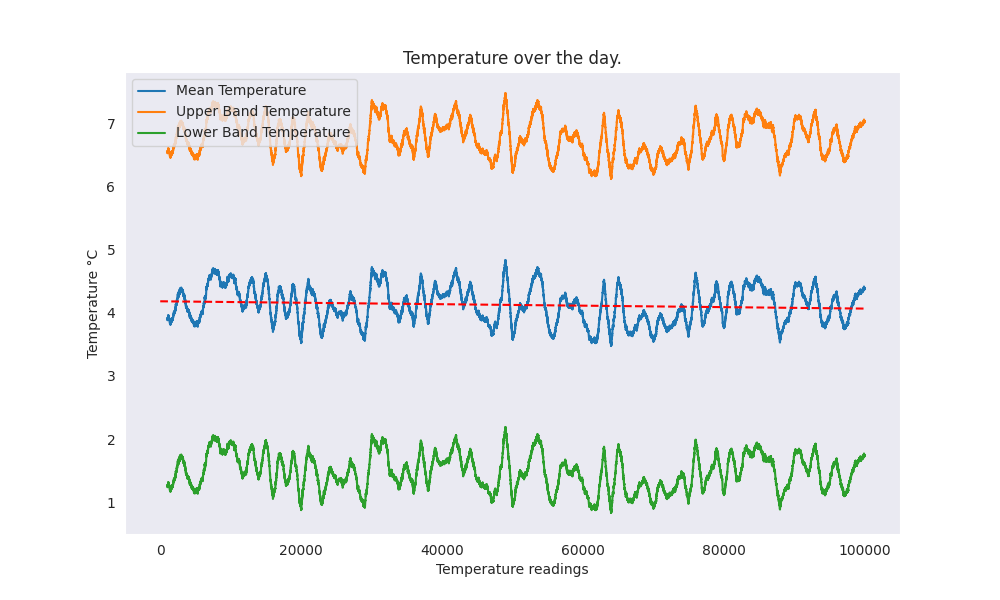
\includegraphics[width=\textwidth/2]{./temp/temperature_plot.png}
        \caption{Temperature over time}
    \end{center}
\end{figure}

%%--------------------%%
\vspace{5mm}
\subsubsection{Humidity}

The humidity average of all the batches during the period was, as the next figure shows.

% Show plot of the temperature average over time
\begin{figure}[H]
    \begin{center}
        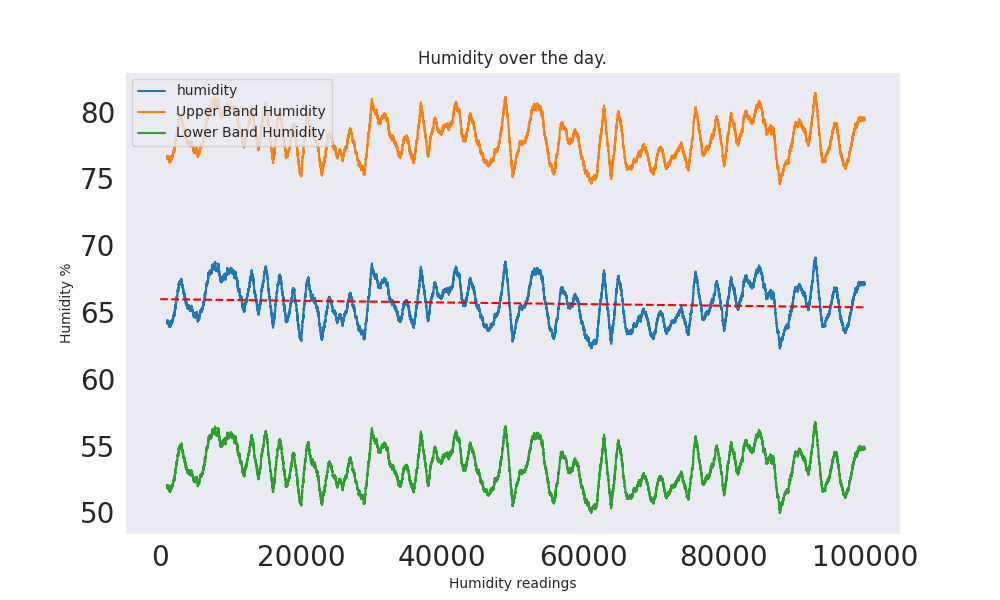
\includegraphics[width=\textwidth/2]{./temp/humidity_plot.png}
        \caption{Humidity over time}
    \end{center}
\end{figure}

%%--------------------%%

\subsubsection{UV Light}

The UV light average of all the batches during the period was, as the next figure shows.

% Show plot of the temperature average over time
\begin{figure}[H]
    \begin{center}
        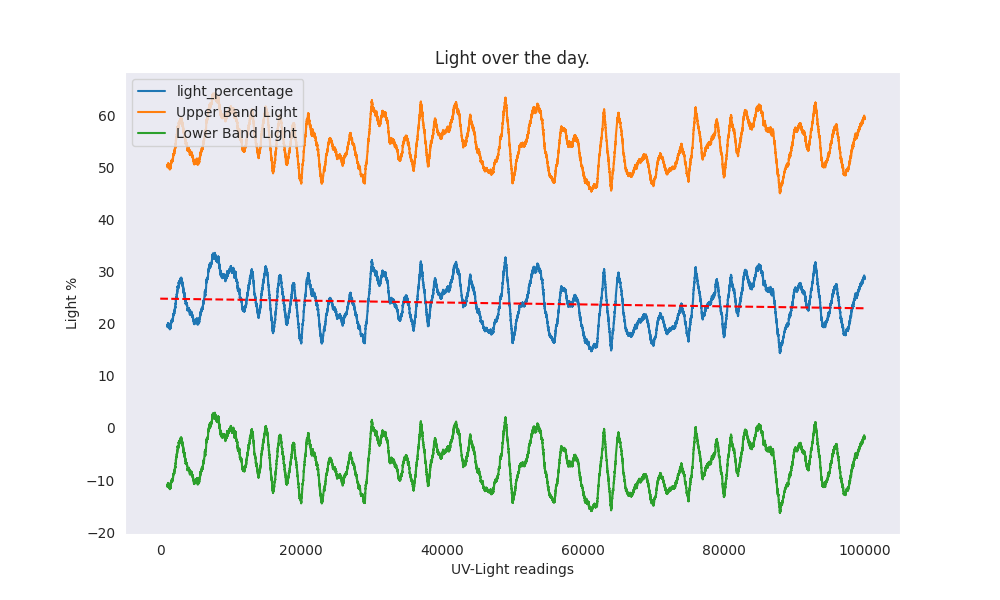
\includegraphics[width=\textwidth/2]{./temp/light_plot.png}
        \caption{UV Light over time}
    \end{center}
\end{figure}

%%--------------------%%

\subsection{Notable Data Points}

The highest and lowest values for the temperature, humidity, and UV light for the day, amongst all batches, are as follows:

\begin{itemize}
    \item \textbf{Temperature:} Highest - {<<HIGHEST_TEMPERATURE>>}, Lowest - {<<LOWEST_TEMPERATURE>>}
    \item \textbf{Humidity:} Highest - {<<HIGHEST_HUMIDITY>>}, Lowest - {<<LOWEST_HUMIDITY>>}
    \item \textbf{UV Light:} Highest - {<<HIGHEST_UV_LIGHT>>}, Lowest - {<<LOWEST_UV_LIGHT>>}
\end{itemize}

%%--------------------%%

\subsection{Individual batches}

\subsubsection{Monitored Batches' Position}

The next table shows the approximate location of the batches monitored during the day.

\begin{table}[ht]
    \centering
    \begin{tabular}{|c|c|}
        \hline
        \textbf{Batch Number} & \textbf{Approximate Location} \\
        \hline
        001 & <<Location 001>> \\
        002 & <<Location 002>> \\
        \hline
        % Add more rows as needed
    \end{tabular}
    \caption{Approximate Locations of Monitored Batches}
    \label{tab:batch_positions}
\end{table}

%%--------------------%%

% \subsubsection{Monitored Batches' Cumulative Transport Time}

% The next table shows an approximation of the time that each batch has been on transport, starting from the moment the censoring module was installed, until now.

% \begin{table}[ht]
%     \centering
%     \begin{tabular}{|c|c|}
%         \hline
%         \textbf{Batch Number} & \textbf{Transport time} \\
%         \hline
%         001 & <<Time 001>> \\
%         002 & <<Time 002>> \\
%         \hline
%         % Add more rows as needed
%     \end{tabular}
%     \caption{Approximate Locations of Monitored Batches}
%     \label{tab:batch_positions}
% \end{table}


%% We may add a section for quick recomendations of action, based on the results of the report

\end{document}
